\section{Parallelization on multiple qunatum devices}
As seen above, minimization of the cost function can be returned to solving the eigenvalues of matrix $G=\sum_{i=1}^Ny_iG_i$, where $N$ is the data size. 
Here, let the data size be $N$ times $M$ again, and consider obtaining the matrix $G$. If $G^{(m)}$ is newly defined as follows, 
$$G^{(m)}=\sum_{i=(m-1)N+1}^{mN}y_iG_i$$
G can be written as $G=\sum_{m=1}^MG^{(m)}$. Thus, if there are $M$ quantum devices, it is possible that $NM$ pieces of data are divided into $M$ equal parts and sent to quantum devices by $N$ pieces, each device calculates $G^{(m)}$, sends the calculation result to the central server, and the central server adds all the matrix $G^{(m)}$ sent to itself to obtain $G$. As can be seen from the above, unlike the gradient-based optimizer \cite{9775600, Qi_2022}, parallelization of this algorithm does not change the progress of learning. Parameters are optimized exactly the same as without parallelization.

\begin{figure}[htb]
    \centering
    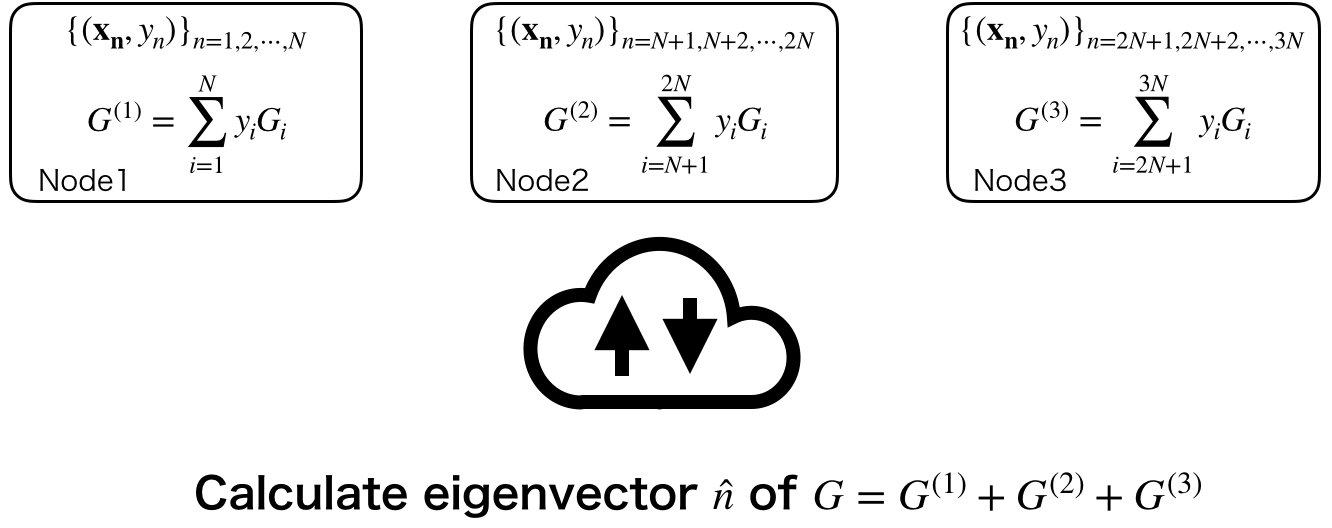
\includegraphics[keepaspectratio, scale=0.5]{method/example.png}
    \caption{Example of parallelization by 3 quantum nodes.}
    \label{fig:example}
\end{figure}